\documentclass[final]{beamer}
\usepackage[size=custom,width=61,height=85,scale=0.9]{beamerposter}
\usetheme{default}
\usepackage{times}
\usepackage{amsmath,amssymb}
\usepackage{booktabs}
\usepackage{graphicx}
\usepackage{xcolor}
\usepackage{tikz}

% ---- Colors ----
\definecolor{gtgold}{HTML}{B3A369}
\definecolor{gtnavy}{HTML}{003057}
\definecolor{negred}{HTML}{D6604D}
\definecolor{posgreen}{HTML}{4DAC26}
\definecolor{lightbg}{HTML}{F5F5F5}

\setbeamercolor{block title}{fg=white,bg=gtnavy}
\setbeamercolor{block body}{fg=black,bg=lightbg}
\setbeamercolor{block alerted title}{fg=white,bg=negred}
\setbeamercolor{block alerted body}{fg=black,bg=negred!8}
\setbeamerfont{block title}{size=\large,series=\bfseries}
\setbeamertemplate{navigation symbols}{}

\newlength{\colwidth}\setlength{\colwidth}{0.46\textwidth}

\begin{document}
\begin{frame}[t]

% ==== TITLE BAR ====
\begin{beamercolorbox}[wd=\textwidth,sep=0.8cm]{block title}
\centering
{\Huge\bfseries Think Less, Code Better:\\[0.2em]
Probing When Chain-of-Thought Hurts and How to Route Around It}\\[0.6em]
{\Large Rajarshi Ghoshal \quad Debadri Basak \quad Salma E.\ Abdelhalim \quad Pratibha K.\ Arora}\\[0.2em]
{\large College of Computing, Georgia Institute of Technology}\\[0.2em]
{\normalsize ICLR 2026 Workshop on Logical Reasoning of Large Language Models}
\end{beamercolorbox}

\vspace{0.6cm}

\begin{columns}[t]

% ==== LEFT COLUMN ====
\begin{column}{\colwidth}

\begin{block}{Motivation}
Chain-of-Thought (CoT) prompting is the default reasoning strategy for LLMs. We test whether it actually helps for \textbf{code generation} using a controlled \textbf{2$\times$2 design}:
\begin{itemize}
    \item 2 architectures $\times$ 2 regimes (base vs.\ instruct)
    \item 3 benchmarks: HumanEval, MBPP, LiveCodeBench
    \item + CodeLlama-7B as a third architecture
\end{itemize}
\end{block}

\vspace{0.5cm}

\begin{alertblock}{\centering Key Finding: CoT Reversal}
\centering
\vspace{0.3em}
For \textbf{Qwen2.5-Coder} on the \textbf{same base architecture}:\\[0.4em]
{\LARGE\color{posgreen}\textbf{Base: CoT helps +13.4\%}} {\large($p<0.001$)}\\[0.3em]
{\LARGE\color{negred}\textbf{Instruct: CoT hurts $-$15.2\%}} {\large($p<0.001$)}\\[0.5em]
\textbf{DeepSeek:} insensitive (all $p>0.2$) \quad \textbf{CodeLlama:} hurt ($-6.7\%$, $p=.022$)\\[0.3em]
\end{alertblock}

\vspace{0.5cm}

\begin{block}{CoT Effect Across Models and Datasets}
\centering
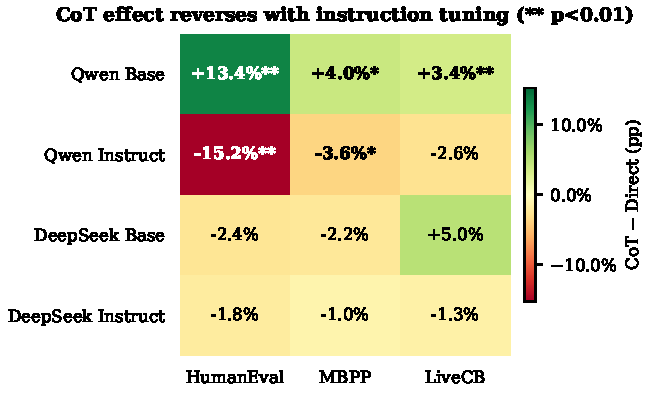
\includegraphics[width=0.88\linewidth]{figures/fig2_cot_reversal.pdf}
\vspace{0.3em}

Green = helps; Red = hurts. $**$\,$p<0.01$. \textbf{Instruction tuning flips the sign.}
\end{block}

\vspace{0.5cm}

\begin{block}{Mechanistic Explanation: Early Encoding}
\centering
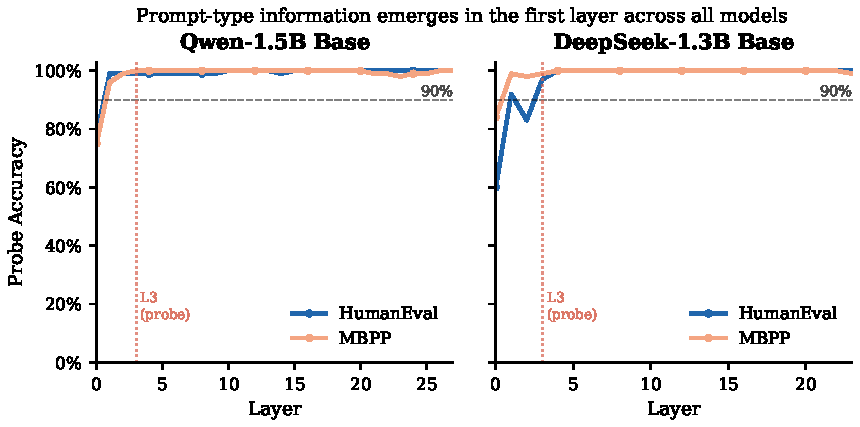
\includegraphics[width=0.88\linewidth]{figures/fig1_tomography.pdf}
\vspace{0.3em}

All models encode prompt type by \textbf{Layer 1--4} ($>$90\%). This is \textbf{universal} --- present whether CoT helps or hurts.

\vspace{0.3em}
\textbf{$\Rightarrow$ Representation $\neq$ interpretation.}\\
Same signal, opposite outcomes depending on training regime.
\end{block}

\end{column}

% ==== RIGHT COLUMN ====
\begin{column}{\colwidth}

\begin{block}{Probe-Guided Style Router}
A lightweight MLP uses early-layer activations to select from \textbf{12 prompt styles} per problem in a single forward pass:

\vspace{0.3em}
\centering
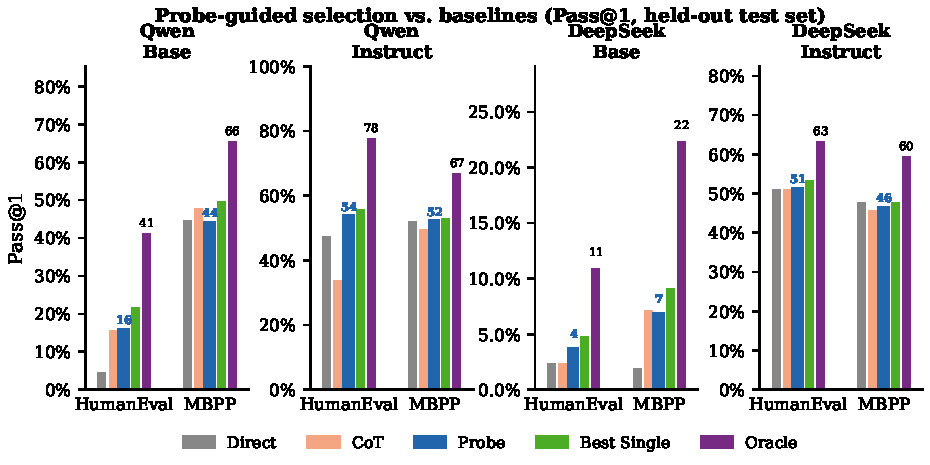
\includegraphics[width=0.88\linewidth]{figures/fig3_strategy_selector.pdf}

\vspace{0.3em}
\begin{tabular}{lcccc}
    \toprule
    \textbf{Setting} & \textbf{Probe} & \textbf{CoT} & \textbf{Best} & $p_{\text{Best}}$ \\
    \midrule
    Qwen Inst./HE & \textbf{53.7} & 34.1 & 56.1 & n.s. \\
    Qwen Inst./MB & 52.0 & 50.0 & 53.2 & n.s. \\
    DS Inst./HE & 51.2 & 51.2 & 53.7 & n.s. \\
    DS Inst./MB & 46.4 & 46.0 & 48.0 & n.s. \\
    \bottomrule
\end{tabular}

\vspace{0.3em}
\flushleft
\textbf{Indistinguishable from best fixed style} in 7/8 settings (McNemar's).\\
Beats CoT where it's most harmful ($p=0.012$, $h=+0.40$).\\
\textbf{84ms overhead} (3.3\%). No prompt engineering needed.
\end{block}

\vspace{0.5cm}

\begin{block}{When Is the Probe Useful?}
\centering
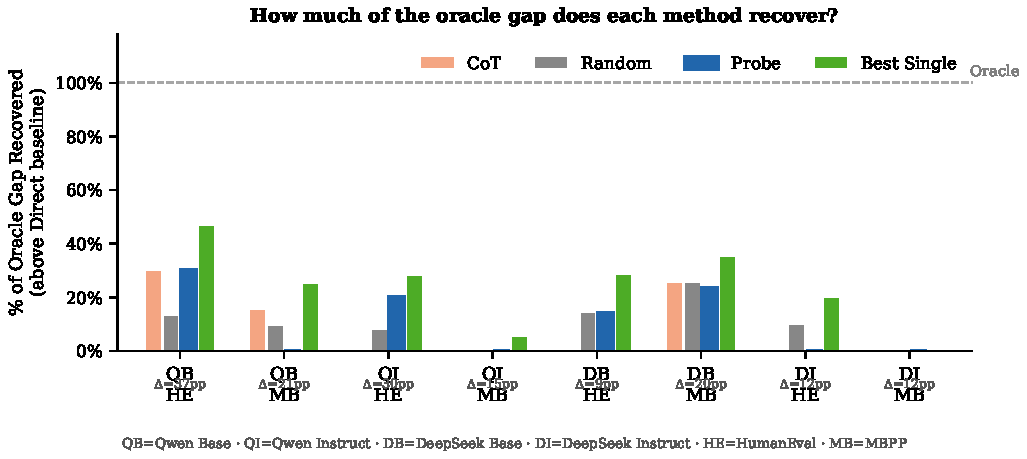
\includegraphics[width=0.80\linewidth]{figures/fig5_oracle_gap.pdf}
\vspace{0.3em}

Probe helps most when \textbf{style variance is high} ($\sigma > 0.04$).\\
When styles perform similarly, probe adds nothing --- but costs nothing.
\end{block}

\vspace{0.5cm}

\begin{block}{Takeaways}
\begin{enumerate}
    \item \textbf{Don't default to CoT} --- it can hurt instruct models by 15pp.
    \item \textbf{CoT sensitivity is architecture-specific} --- not universal.
    \item \textbf{Models encode prompt type by Layer 1--4} --- early and universal.
    \item \textbf{A cheap activation probe matches the best fixed style} --- no prompt engineering.
\end{enumerate}
\end{block}

\end{column}
\end{columns}

\end{frame}
\end{document}
